% main.tex -- NeurIPS 2026 Datasets & Benchmarks Track submission
% Anonymized for double-blind review.
%
% IMPORTANT: this submission uses a PLACEHOLDER neurips_data_2026.sty.
% Replace with the official style file from https://nips.cc/Conferences/2026
% when the D&B CFP drops, and re-run `pdflatex` to regenerate.
%
% Build:
%   pdflatex main && bibtex main && pdflatex main && pdflatex main

\documentclass{article}

% Default = anonymous (double-blind). Pass [final] for camera-ready.
\usepackage{neurips_data_2026}

\usepackage[T1]{fontenc}
\usepackage[utf8]{inputenc}
\usepackage{amsmath,amssymb}
\usepackage{microtype}
\usepackage{textcomp}
\usepackage{array}
\usepackage{caption}

\graphicspath{{figures/}}

\title{\bfseries RAG-Eval-LLM-Judge: A 5-Family, 9-Judge Cross-Family LLM-Judge Agreement Benchmark for Institutional Retrieval}

\author{\textit{[anonymized for double-blind review]}}

\begin{document}
\maketitle

\begin{abstract}
We release \textbf{RAG-Eval-LLM-Judge}, a fully reproducible benchmark suite for studying inter-LLM-judge agreement on bounded ordinal information-retrieval relevance judgment, plus a reference 9-judge dataset that demonstrates its use. The benchmark addresses a methodological gap that no current public artifact closes simultaneously: a \textbf{five-family} pairwise quadratic-weighted Cohen's $\kappa$ matrix on a \textbf{bounded 0--3 ordinal} rubric at \textbf{$\geq$~500 paired observations}, with \textbf{within-family controls} and \textbf{open-weight peers as first-class participants}. Our reference run scores 9 LLM judges (Anthropic $\times$2, OpenAI $\times$2, Google-commercial $\times$2, DeepSeek $\times$1, Open-weight $\times$2) on \textbf{570 query-document pairs from a US-public-university institutional repository (97k full-text PDFs)} plus \textbf{1{,}137 pairs across three external public corpora with NIST/BEIR human qrels} (TREC RAG 2024, TREC-COVID, BEIR scifact). The release contains 9{,}963 individual LLM-judge score records, a 1{,}500-line Python harness, a programmatic verifier (62 numerical checks), a 25-test pytest suite, Croissant 1.0 metadata, a HuggingFace data card, plus pre-computed bootstrap 95\% CIs, Gwet AC2, intra-judge self-consistency, bias diagnostics, and an UMBRELA single-judge baseline. Total reproduction cost from a clean checkout is $\sim$\$95 in paid API spend and $\sim$13 hours of wall time, replacing an institution-specific IRB human-rater study (estimated \$1{,}500--3{,}000 / 6--12 weeks). The headline empirical finding the dataset establishes---that a cross-organization open-weight pair (Qwen 3.6 Plus + Gemma 4 26B) \textbf{matches} the cross-family commercial reasoning ceiling at point-estimate $\kappa = 0.80$ (95\% CI [0.76, 0.83], overlapping the commercial reasoning pair's [0.75, 0.82]) and \textbf{clearly exceeds every commercial within-family pair} (non-overlapping CIs)---supports an ensemble deployment recommendation for sovereign-cloud and privacy-conservative institutions. Repository: \emph{[anonymous URL]}.
\end{abstract}

\section{Introduction}\label{sec:intro}

Modern retrieval-augmented generation (RAG) systems sit on top of vector retrievers tuned over institutional corpora---academic libraries, parliamentary archives, medical records, legal collections. Practitioners want to answer ``is this retrieval good?''---but they hit three blockers: there is no gold relevance set (TREC-style ground truth requires hundreds of expert hours per topic), generic IR benchmarks (BEIR, MS-MARCO) do not transfer, and the canonical workaround---\textbf{LLM-as-Judge} \citep{zheng2023judge,faggioli2023perspectives,rahmani2024judges,upadhyay2024umbrela}---surfaces a downstream question that has not been answered by a public reproducible artifact: \textbf{which LLM judge?}

The recent literature has begun to address this question, but published comparisons cover either: (a) a single provider family \citep{balog2025rankersjudges,farzi2025umbrela_other}, (b) two-family pairs without ordinal weighting (\citealp{thakur2025trecragsupport}: $\kappa = 0.60$ for GPT-4o vs.\ Llama-3.1-405B on 537 unweighted pairs), or (c) judge-vs-human only \citep{han2025judgesverdict}. None---to our knowledge---provides a \textbf{public, reproducible artifact} containing simultaneously: a multi-family pairwise $\kappa$ matrix, within-family controls, open-weight peers as first-class participants, a bounded ordinal rubric, $\geq$~500 paired observations, and external validation against public NIST / BEIR human qrels.

We close that gap with \textbf{RAG-Eval-LLM-Judge}, a complete reproducible release covering all six axes. The within-corpus reference run is on \textbf{570 pairs} from a US-public-university institutional DSpace repository; external validation runs cover \textbf{537 pairs from TREC RAG 2024}, \textbf{300 from BEIR scifact}, and \textbf{300 from TREC-COVID}, all using identical 9-judge slate, identical rubric, identical pipeline.

\textbf{Contributions.}
\begin{itemize}
\item \textbf{C1.} A reproducible 9{,}963-record cross-family LLM-judge agreement dataset spanning four corpora (one institutional, three public).
\item \textbf{C2.} An open-source Python harness covering scoring, multi-corpus validation, MS MARCO v2.1 streaming extraction, and the cross-run merge---the entire experiment re-runs from a clean checkout in $\sim$13 hours wall and $\sim$\$95 paid-API spend.
\item \textbf{C3.} A programmatic claim verifier (62 numerical checks) and a 25-test pytest suite, both runnable in $<$ 5 seconds, that assert every number in the companion paper against the shipped JSONs.
\item \textbf{C4.} A Croissant 1.0 metadata document and HuggingFace-style data card, supporting machine-readable dataset discovery and ML-platform integration.
\item \textbf{C5.} A community \textbf{disclosure-template} standard for LLM-judged retrieval reporting: ``nDCG@10 = X.XX via [family]/[model]/[reasoning-config], $N$ pairs, DATE'' (Fig.~\ref{fig:disclosure}).
\end{itemize}

\section{Related Work and Position in the Benchmark Landscape}

\paragraph{LLM-as-Judge for IR.} \citet{faggioli2023perspectives}, \citet{rahmani2024judges}, and UMBRELA \citep{upadhyay2024umbrela} established LLMs as practical IR-relevance assessors. UMBRELA in particular has been deployed at TREC scale on the 2024 RAG track and is the closest single-judge baseline to our work; we run it as an explicit comparison point (\S\ref{sec:results}).

\paragraph{The 2025 inter-LLM-judge agreement cluster.} A 2025 cluster has begun reporting inter-LLM agreement on relevance---\citet{balog2025rankersjudges} (single-family), \citet{thakur2025trecragsupport} (two-family pair without ordinal weighting), \citet{han2025judgesverdict} (judge-vs-human only). None provides the combination we ship. Parallel evidence from educational measurement \citep{jiao2026essayraters} shows frontier LLMs converging on quadratic-weighted $\kappa$ with humans on 0--$N$ ordinal scoring, supporting the cross-domain plausibility of our results.

\paragraph{Existing IR benchmarks vs.\ this dataset.} BEIR \citep{thakur2021beir} is the dominant public IR benchmark suite but treats each LLM judge as a single-output black box; it does not surface inter-judge agreement structure. The TREC RAG 2024 track \citep{macavaney2025trec_rag} publishes NIST human qrels but has \textbf{no published inter-LLM-judge agreement matrix} at our scale. RAGAS \citep{es2024ragas} and similar frameworks report agreement against humans, not pairwise across LLMs. Our release \textbf{complements} rather than competes with these: it stress-tests the LLM-as-Judge primitive itself by pitting nine of them against each other and against the human qrels these other benchmarks use.

\section{Dataset Description}

\subsection{Reference judge slate (9 judges, 5 families)}

\begin{table}[h]
\centering\small
\caption{Judge slate. Within-family pairs: Anthropic (1$\leftrightarrow$2), OpenAI (3$\leftrightarrow$4), Google-commercial (5$\leftrightarrow$6), Open-weight cross-organization (8$\leftrightarrow$9). DeepSeek V4 Flash dropped due to OpenRouter free-tier 429 throttling. Versions pinned at 2026-04-25.}
\label{tab:judges}
\begin{tabular}{@{}clllc@{}}
\toprule
\# & Judge & Family & Reasoning & API route \\
\midrule
1 & Claude Opus 4.7 & Anthropic & yes & OpenRouter \\
2 & Claude Sonnet 4.6 & Anthropic & yes & OpenRouter \\
3 & GPT-5.5 (reasoning=low) & OpenAI & yes & OpenAI direct \\
4 & GPT-4o (chat) & OpenAI & no & OpenAI direct \\
5 & Gemini 3.1 Pro Preview & Google-commercial & yes (thinking) & OpenRouter \\
6 & Gemini 2.5 Pro & Google-commercial & yes (thinking) & OpenRouter \\
7 & DeepSeek V4 Pro & DeepSeek & yes & OpenRouter \\
8 & Qwen 3.6 Plus & Open-weight & no & OpenRouter \\
9 & Gemma 4 26B & Open-weight & no & OpenRouter \\
\bottomrule
\end{tabular}
\end{table}

\subsection{Within-corpus dataset (570 pairs, 5{,}130 records)}\label{sec:within}

\textbf{Corpus.} A US-public-university DSpace institutional repository: 97{,}441 full-text PDFs $\rightarrow$ 1.03M chunks ($\leq$500 words, 100-word overlap), embedded with Google Vertex \texttt{text-embedding-005} in Qdrant 1.13 HNSW. \textbf{Queries:} 57 from a corpus-faithful query-synthesis method, balanced across factoid/methodological/comparative/author-style intents over 20 topic clusters. \textbf{Pairs:} top-10 retrieval per query $\rightarrow$ 570 (query, document) pairs.

\textbf{Released artifacts} (in \texttt{results/within\_corpus/}): 9 per-judge JSONs ($\sim$340~KB each) holding the full 57-query $\times$ 10-retrieval structure; 1 merged multijudge JSON ($\sim$8~KB) with aggregates + 9$\times$9 pairwise $\kappa$ matrix; schema documented in \texttt{results/within\_corpus/README.md}. Retrieval determinism is verified by every per-judge file sharing the same \texttt{(query\_id, rank, point\_id)} triple sequence.

\subsection{External-validation datasets (1{,}137 pairs, 4{,}833 valid records)}\label{sec:external}

\begin{table}[h]
\centering\small
\caption{External-validation corpora and sample method.}
\label{tab:external}
\begin{tabular}{@{}lrlll@{}}
\toprule
Corpus & $n$ & Sample method & Qrels source & Format \\
\midrule
TREC RAG 2024 & 537 & Stratified-balanced 135/134/134/134 across 0/1/2/3 & NIST 2024 retrieval-qrels & 0--3 ordinal \\
TREC-COVID & 300 & First 300 from BEIR \texttt{GenericDataLoader} & BEIR-distributed & 0/1/2 $\rightarrow$ 0/2/3 \\
BEIR scifact & 300 & First 300 from BEIR \texttt{GenericDataLoader} & BEIR scifact & binary $\rightarrow$ 0/3 \\
\bottomrule
\end{tabular}
\end{table}

External-validation files use a flat shape: \texttt{pair\_index} ($n$ tuples), \texttt{human\_scores} (length $n$), \texttt{per\_judge\_scores} (dict of length-$n$ score arrays per judge label), \texttt{per\_judge\_metadata}. \texttt{pair\_index} and all score arrays are aligned positionally.

\subsection{Intra-judge self-consistency subset (1{,}350 records)}

50 pairs $\times$ 9 judges $\times$ 3 runs (\texttt{results/intra\_judge\_consistency.json}). Pairs are sampled deterministically (\texttt{random.seed(42)}) from the 537-pair TREC RAG 2024 stratified set. Mean intra-judge $\kappa$ across 9 judges = \textbf{0.93}, range 0.89 (Qwen) to 1.00 (Opus 4.7, Gemini 3.1 Prev, Gemini 2.5 Pro). All 9 judges have intra-$\kappa$ $>$ $\kappa$-vs-human ($\Delta$ range $+$0.51 to $+$0.70); no judge in the slate is ``Rating Roulette unstable.''

\subsection{UMBRELA single-judge baseline}

\texttt{results/umbrela\_baseline\_trec\_rag\_2024.json}: GPT-4o + UMBRELA verbatim prompt \citep{upadhyay2024umbrela} on the same 537-pair TREC RAG 2024 sample, for direct comparison against our 9-judge ensemble. Result: $\kappa$ vs.\ human = \textbf{0.4265}, $n_{valid}$ = 537/537 (100\%), 1.7~min wall, \$0.30. Two independent runs at temperature 0.0 produced 0.4265 and 0.4387---a 0.012 $\kappa$ jitter that motivates the intra-judge subset.

\subsection{Pre-computed analytical artifacts}

\textbf{\texttt{bootstrap\_kappa\_cis.json}} (1000-resample 95\% CIs, seed=42); \textbf{\texttt{gwet\_ac2\_alongside\_kappa.json}} (Gwet AC2 alongside Cohen $\kappa$ \citep{gwet2008}); \textbf{\texttt{bias\_diagnostics.json}} (5$\times$5 family conditional-mean matrix + per-judge marginal score distributions); \textbf{\texttt{verification\_log.txt}} (62 programmatic checks, all passing).

\section{Benchmark Methodology}

\textbf{Rubric.} 0~=~irrelevant, 1~=~topical, 2~=~partial, 3~=~fully answers. Calibrated at prompt time with five worked examples. Documents truncated to 1{,}500 chars \citep{saito2023verbosity}. Temperature 0.0.

\textbf{Pipeline.} \texttt{src/eval\_llm\_judge.py} fans the 9 judges per pair via \texttt{ThreadPoolExecutor}, retries on transient errors with exponential backoff, saves per-judge JSONs plus a combined $\kappa$ matrix. Two-phase deployment supported: 7-judge frontier preset + 2-judge open-weight supplement, merged with retrieval-determinism verification.

\textbf{Metrics.} Per-judge nDCG@10, P@5 ($s \geq 2$), MRR. Inter-judge agreement is pairwise quadratic-weighted Cohen's $\kappa$ \citep{thakur2024judges,cohen1968,fleiss1971}, interpreted via Landis--Koch bands \citep{landis1977}. Gwet AC2 reported alongside for triangulation under marginal-skew. Where a judge returned a missing/unparseable score, we exclude that pair from the judge's mean and from any $\kappa$ pair involving that judge. KL divergence on score marginals computed per \citet{kullback1951}.

\textbf{Ensemble convention.} All ensemble medians use the upper-middle convention: \texttt{sorted\_votes[n // 2]}, applied uniformly across all corpora.

\section{Validation Results (illustrative use case)}\label{sec:results}

The following are headline numbers the dataset enables; full mechanistic and limitations analysis is in the companion long paper.

\begin{figure}[h]
\centering
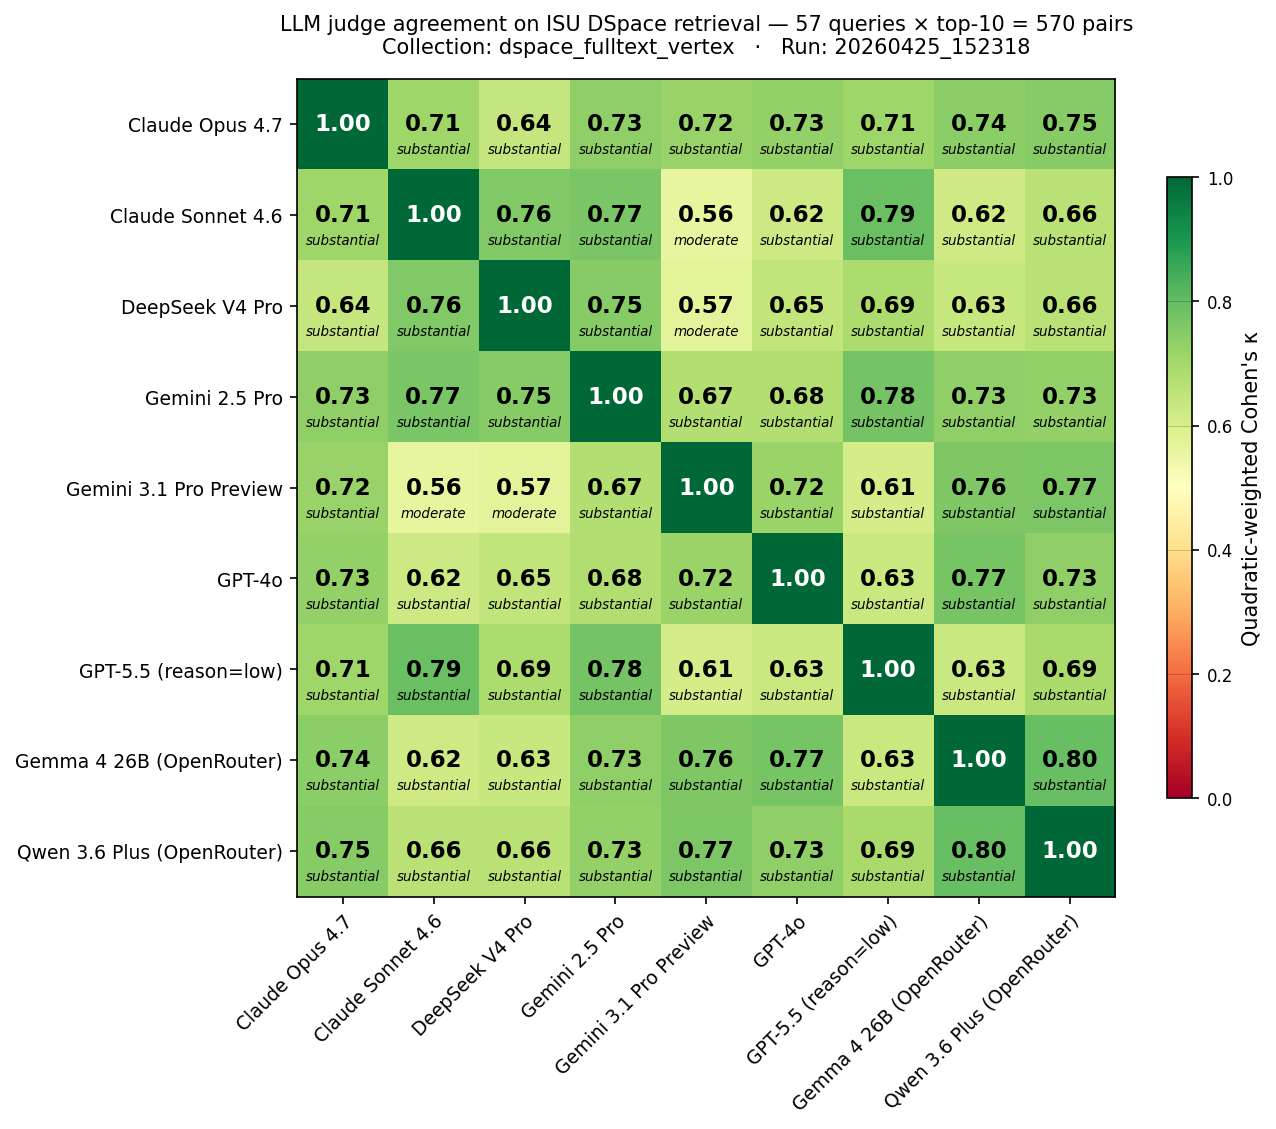
\includegraphics[width=0.92\linewidth]{kappa_matrix_9judge.png}
\caption{Pairwise quadratic-weighted Cohen's $\kappa$ on 570 institutional-repository pairs. Two emergent calibration clusters; matrix-max $\kappa = 0.80$ between Qwen 3.6 Plus and Gemma 4 26B (cross-organization Open-weight); cross-family commercial ceiling 0.79 (Sonnet $\leftrightarrow$ GPT-5.5). 95\% CIs overlap heavily (see Table~\ref{tab:within}).}
\label{fig:kappa}
\end{figure}

\begin{table}[h]
\centering\small
\caption{Within-corpus 9$\times$9 $\kappa$ matrix selected cells with bootstrap 95\% CIs (1000 resamples, seed=42). Qwen$\leftrightarrow$Gemma 4 is the point-estimate matrix-max but the CI overlaps Sonnet$\leftrightarrow$GPT-5.5; the robust empirical claim is that the cross-organization Open-weight pair clearly \emph{exceeds every commercial within-family pair} (non-overlapping CIs).}
\label{tab:within}
\begin{tabular}{@{}lrl@{}}
\toprule
Pair & $\kappa$ & 95\% CI \\
\midrule
Qwen $\leftrightarrow$ Gemma 4 (cross-org Open-weight) & \textbf{0.80} & [0.76, 0.83] \\
Sonnet $\leftrightarrow$ GPT-5.5 (cross-family commercial) & 0.79 & [0.75, 0.82] \\
Anthropic Opus $\leftrightarrow$ Sonnet (within-family) & 0.71 & [0.67, 0.74] \\
Google Gem 3.1 $\leftrightarrow$ Gem 2.5 (within-family) & 0.67 & [0.56, 0.77] \\
OpenAI GPT-5.5 $\leftrightarrow$ GPT-4o (within-family) & 0.63 & [0.59, 0.67] \\
Sonnet $\leftrightarrow$ DSV4 Pro (cross-family) & 0.76 & [0.73, 0.79] \\
\bottomrule
\end{tabular}
\end{table}

Within-cluster mean $\kappa$ (0.74) exceeds cross-cluster mean $\kappa$ (0.68) by 0.06 (Welch $t = 3.45$, $p = 0.002$ two-sided; Mann-Whitney U one-sided $p = 0.004$). \textbf{The same 570 retrieved documents yield nDCG@10 between 0.45 (Gemini 3.1 Prev) and 0.86 (Sonnet 4.6)---a 1.9$\times$ spread driven entirely by judge selection}, which is the empirical hook for the disclosure-template proposal (Fig.~\ref{fig:disclosure}).

\begin{figure}[h]
\centering
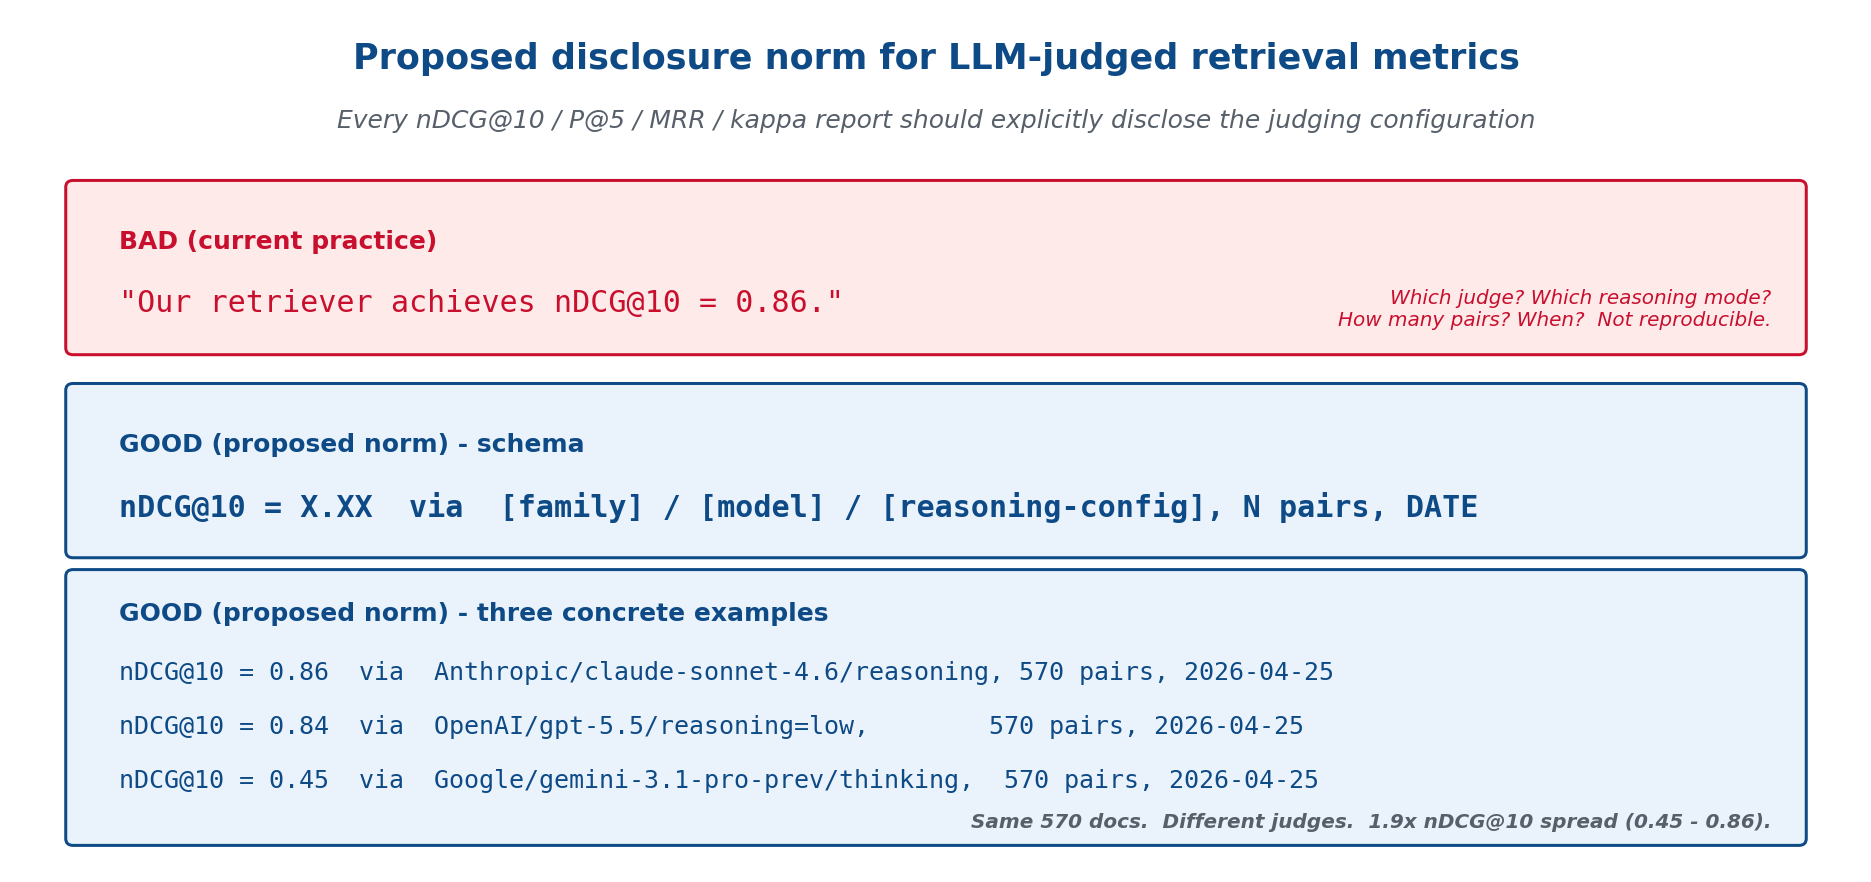
\includegraphics[width=0.95\linewidth]{disclosure_template.png}
\caption{Proposed community disclosure-template standard for LLM-judged retrieval reporting. The same 570 documents yield nDCG@10 = 0.86 under one judge configuration and 0.45 under another; without disclosure, ``our retriever scores 0.86'' is not a comparable measurement.}
\label{fig:disclosure}
\end{figure}

\subsection{External validation against NIST / BEIR human qrels}

\begin{table}[h]
\centering\small
\caption{External validation per-corpus ensemble $\kappa$ (with 95\% bootstrap CI) vs.\ NIST/BEIR human qrels. UMBRELA single-judge baseline shown for comparison on the TREC RAG 2024 sample.}
\label{tab:external_results}
\begin{tabular}{@{}lrll@{}}
\toprule
Corpus / configuration & $\kappa$ vs.\ human & 95\% CI & Landis--Koch \\
\midrule
TREC RAG 2024 (9-judge ensemble) & \textbf{0.4941} & [0.43, 0.56] & moderate, near-substantial \\
TREC RAG 2024 (7-judge frontier ensemble) & 0.5187 & [0.46, 0.58] & moderate-substantial \\
TREC-COVID (9-judge ensemble) & 0.3447 & [0.24, 0.45] & fair, near-moderate \\
TREC-COVID (7-judge frontier ensemble) & 0.4462 & [0.35, 0.53] & moderate \\
BEIR scifact (9-judge ensemble precision-at-$\geq$2) & 65.7\% & --- & ($\kappa$ undefined) \\
\midrule
\textbf{UMBRELA single-judge baseline (TREC RAG 2024)} & 0.4265 & --- & moderate \\
\textbf{Our single best (Sonnet 4.6, TREC RAG 2024)} & 0.5123 & --- & moderate-substantial \\
\bottomrule
\end{tabular}
\end{table}

Both ensembles + best single judge outperform the UMBRELA single-judge baseline by 0.07--0.09 $\kappa$, supporting the methodology contribution as a slate + ensemble (not prompt) advance.

\subsection{Coverage divergence and the always-works subset}\label{sec:coverage}

\begin{table}[h]
\centering\small
\caption{Per-judge coverage on the three external corpora (\% pairs returning a parseable score). The \emph{always-works 6-judge subset} ($\geq$95\% on all three) is Anthropic + OpenAI + Qwen + Gemma---the 2 cheapest open-weight judges make this subset.}
\label{tab:coverage}
\begin{tabular}{@{}lrrr@{}}
\toprule
Judge & TREC RAG 2024 & BEIR scifact & TREC-COVID \\
\midrule
GPT-5.5, GPT-4o, Anthropic, Qwen, Gemma & 100\% & $\geq$95\% & $\geq$84\% \\
DeepSeek V4 Pro & 39\% & 84\% & 83\% \\
Gemini 3.1 Pro Preview & 24\% & 60\% & 44\% \\
Gemini 2.5 Pro & 17\% & 86\% & 6\% \\
\bottomrule
\end{tabular}
\end{table}

\subsection{Mechanism + bias diagnostics summary}

\begin{figure}[h]
\centering
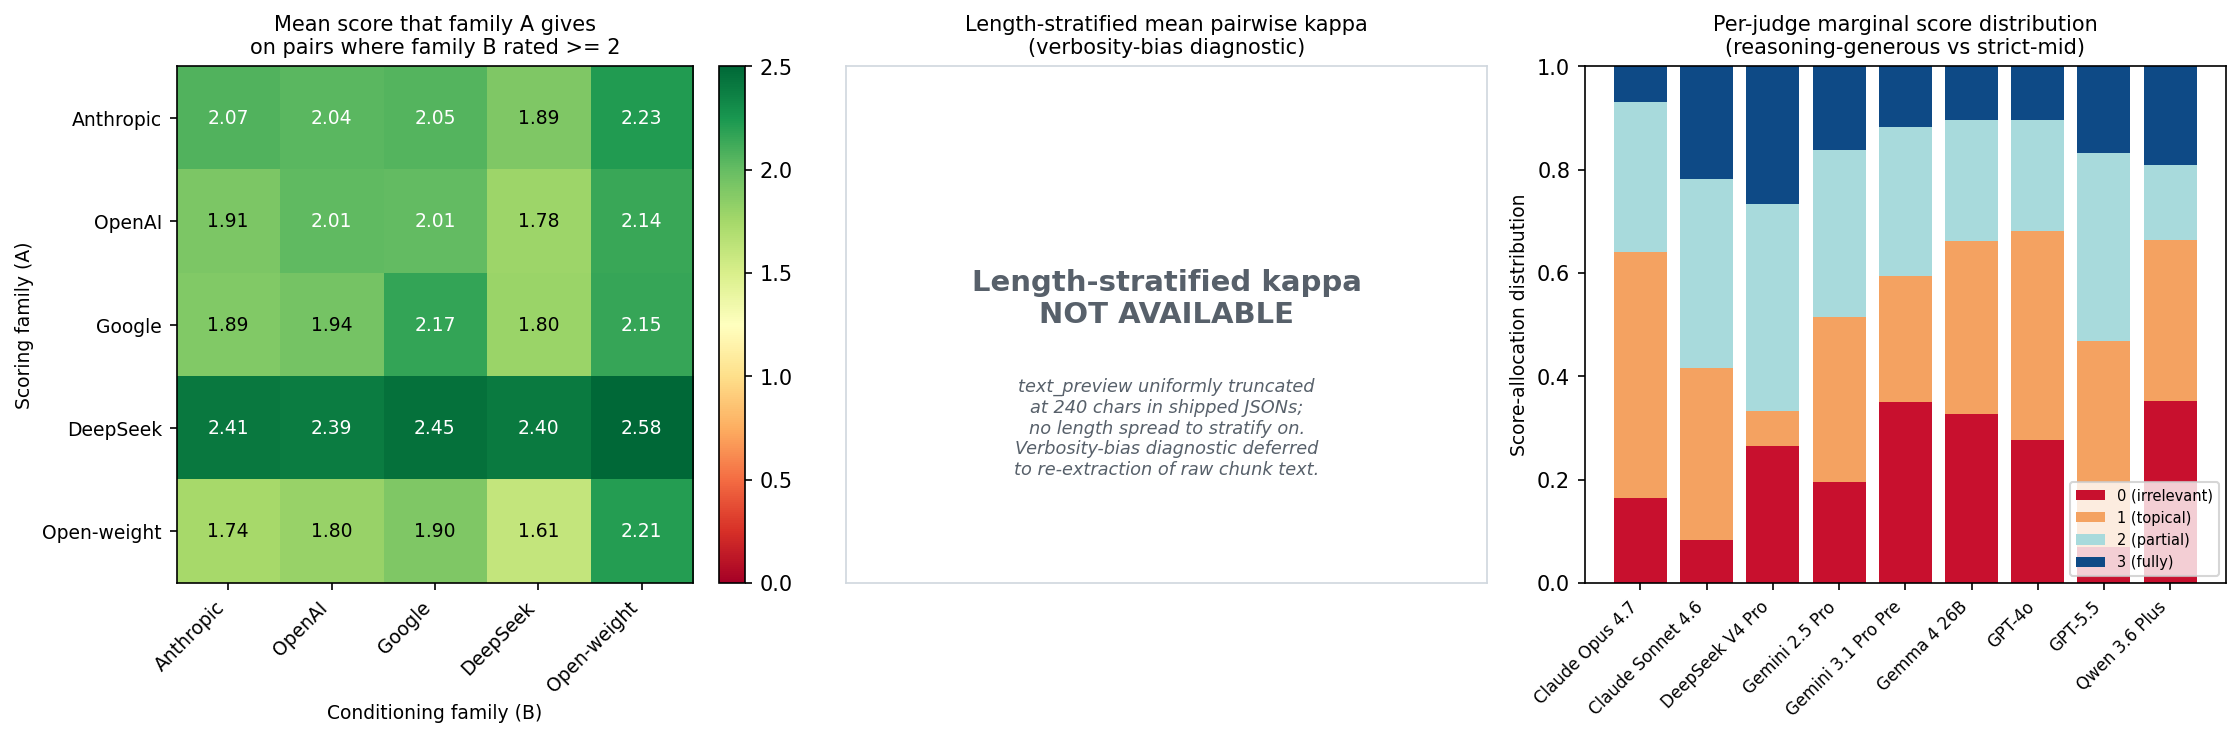
\includegraphics[width=\linewidth]{bias_diagnostics_panel.png}
\caption{Bias diagnostics. Left: 5$\times$5 family conditional-mean matrix---no family's diagonal dominates its row; the pattern is calibration drift, not self-preference. Center: length-stratified $\kappa$ skipped (uniform truncation in stored previews; full diagnostic deferred). Right: per-judge marginal score distributions, visualizing the three calibration clusters (reasoning-generous, strict-mid, Gemini outliers) directly.}
\label{fig:bias}
\end{figure}

A joint-distribution decomposition of $\kappa$ into dispersion (the quadratic-disagreement weight, which appears in the $\kappa$ formula \emph{by construction}) and effective rank (a singular-value summary of the 4$\times$4 confusion matrix) recovers $R^2 = 0.928$ across the 36 unique judge pairs. The high $R^2$ is partly mathematical---synthetic-pair simulation confirms $R^2 \approx 0.998$ in the limit purely from the $\kappa$ formula's weighting structure. The empirically interesting result, descriptively consistent with full mediation in the spirit of \citet{baronkenny1986} and \citet{mackinnon2007}, is that structural factors (provider, reasoning-mode, model class) add $\leq 0.005$ incremental $R^2$ above the decomposition. The shared-tokenizer hypothesis is refuted: Qwen$\leftrightarrow$Gemma 4 vocabulary Jaccard $= 0.066$ (lowest in slate) yet $\kappa = 0.80$ (matrix-highest); convergence is at the decision-making layer, not the tokenizer. Gwet AC2 runs $\approx +0.25$ above Cohen $\kappa$ across the slate, consistent with marginal skew toward the lower ordinal categories (kappa paradox).

\section{Reproducibility}\label{sec:repro}

Full reproduction from a clean checkout requires Python 3.11+, $\sim$1~GB disk, and API keys for OpenAI + OpenRouter ($\sim$\$95 total spend; $\sim$13~hours wall).

\begin{verbatim}
git clone <ANONYMOUS REPO URL>
cd RAG-Eval-LLM-Judge
pip install -r requirements.txt
cp .env.template .env  # fill in OPENAI_API_KEY + OPENROUTER_API_KEY

# Step 0 - verify shipped numerical claims (free, ~3 sec)
py -3 -X utf8 src/verify_paper_claims.py
# -> 62 pass / 0 fail / 0 warn

# Step 1 - external validation harness end-to-end (~$50, ~7.5 h)
py -3 -X utf8 src/validate_against_trec.py \
    --corpus trec-rag-2024 --judge-preset p4-frontier --max-pairs 537
py -3 -X utf8 src/validate_against_trec.py \
    --corpus trec-rag-2024 --judge-preset p4-supplement-openweight --max-pairs 537
py -3 -X utf8 src/validate_against_trec.py --analyze trec-rag-2024
# -> ensemble_median kappa = 0.4941 (matches shipped value to 1e-4)

# Step 2 - UMBRELA single-judge baseline (~$0.30, ~2 min)
py -3 -X utf8 src/run_umbrela_baseline.py
# -> kappa vs human = 0.4265

# Step 3 - intra-judge self-consistency (~$15, ~18 min)
py -3 -X utf8 src/intra_judge_consistency.py

# Step 4 - bootstrap CIs + Gwet AC2 + bias diagnostics (free, < 1 min)
py -3 -X utf8 src/bootstrap_kappa_cis.py
py -3 -X utf8 src/compute_gwet_ac2.py
py -3 -X utf8 src/bias_diagnostics.py

# Step 5 - pytest test suite (free, ~1.5 sec)
py -3 -m pytest -q
# -> 25 passed
\end{verbatim}

\section{Maintenance and Evolution}

\textbf{Versioning.} Released as v1.0. Major bumps for substantial corpus additions (e.g., LLMJudge 2025 benchmark, TREC RAG 2025 replication when qrels publish); minor for additional analyses on existing corpora; patch for numerical errata. \textbf{Maintenance commitment.} Issues responded within 30 days; pull requests reviewed within 14 days for trivial fixes and 60 days for substantive additions. \textbf{Hosting.} GitHub (primary). Zenodo mirror with DOI planned at camera-ready. \textbf{Roadmap.} TREC RAG 2025 replication (when 2025 NIST qrels publish; the same MS MARCO v2.1 passage extractor works unchanged); self-hosted open-weight replication; provenance-labeled documents for a strict self-preference test \citep{panickssery2024self}; additional public corpora (LLMJudge benchmark, TREC-COVID full set when expanded qrels publish).

\section{Ethics, Licensing, and Responsible Use}

\textbf{Licensing.} MIT for code; CC-BY-4.0 for data/figures/papers. Third-party redistributed inputs (MS MARCO v2.1 passages, NIST TREC RAG 2024 qrels) retain their original licenses; we redistribute only score arrays and metadata derived under terms of fair-use research.

\textbf{Privacy and consent.} The institutional repository content is publicly published academic material (theses, conference proceedings, journal volumes); no PII beyond author names that already appear on public publications. TREC RAG 2024 / TREC-COVID / BEIR scifact: pre-published by NIST / BEIR consortium. API responses obtained under provider terms of service for research use; we redistribute only integer/null scores, not raw API response text.

\textbf{Intended uses.} Reproducibility of LLM-as-Judge for IR meta-evaluation; methodology research on inter-rater agreement, bias, and ensemble design; practitioner guidance on judge selection. \textbf{Out-of-scope.} The dataset is \emph{not} a substitute for human-rater studies on sensitive corpora (medical, legal, security-critical); use it as a methodology-vetting tool, not a deployment ground-truth. The ``always-works 6-judge subset'' finding applies to the three external corpora measured; institutions deploying on substantially different content (mathematical reasoning, code, multilingual non-English) should validate before relying on the recommendation.

\section{Limitations}

Single internal corpus for the within-corpus 9$\times$9 matrix; stratified-balanced TREC RAG 2024 sample is not directly comparable to natural-distribution-proportional samples; DeepSeek V4 Flash dropped due to throttling (incomplete within-DeepSeek pair); aggregate metrics treat \texttt{null} as 0 with valid-only means alongside; the mechanism's $R^2 = 0.928$ between $\kappa$ and dispersion+rank is partly mathematical (full disclosure in the companion long paper); the open-weight cost claim uses API routing rather than on-prem inference, so the policy claim about sovereign-cloud is provisional pending self-hosted replication; intra-judge $\kappa$ on $n = 50$ pairs has wide bootstrap CIs (point-estimate ranking, not material-effect claims).

\section{Conclusion}

We release a complete reproducible benchmark + reference dataset for studying inter-LLM-judge agreement on bounded ordinal IR relevance judgment. The release closes a six-axis gap (multi-family $\times$ within-family controls $\times$ open-weight first-class $\times$ bounded ordinal $\times$ $\geq$~500 obs $\times$ external validation) that no current public artifact addresses simultaneously. The accompanying empirical findings---cross-family $\kappa \geq 0.75$ convergence, cross-organization open-weight matching the commercial reasoning ceiling, kappa-paradox-robust triangulation via Gwet AC2, and an ``always-works 6-judge subset'' recommendation---are documented as illustrative use cases of what the dataset enables. Full mechanism analysis and limitations: companion long paper.

\section*{Acknowledgments}

\textit{[redacted for double-blind review; will be restored at camera-ready]}

\bibliographystyle{plainnat}
\bibliography{references}

\appendix

\section{Croissant 1.0 metadata}\label{app:croissant}

The repository's \texttt{croissant.json} provides Croissant 1.0 JSON-LD metadata with 11 distribution \texttt{FileObject}/\texttt{FileSet} entries and 2 \texttt{RecordSet} schemas for the external-validation and within-corpus record types, supporting machine-readable dataset discovery and ML-platform integration.

\section{HuggingFace data card}\label{app:datacard}

The repository's \texttt{DATA\_CARD.md} provides a HuggingFace-style data card with YAML frontmatter declaring 8 dataset configurations and full sections covering: dataset summary, supported tasks, structure (per-judge JSONs + external-validation flat format + intra-judge subset), splits, curation rationale, source data, annotations, sensitive info, social impact, biases, limitations, citation, license, maintenance plan.

\section{Verification log}\label{app:verifier}

\texttt{src/verify\_paper\_claims.py} runs 62 numerical checks against the shipped JSONs in $<$~5~seconds. The shipped \texttt{results/verification\_log.txt} captures the latest run with all 62 checks passing.

\section{Cost and wall-time accounting}\label{app:cost}

\begin{table}[h]
\centering\small
\caption{Reproduction-cost and wall-time accounting from a clean checkout.}
\label{tab:cost}
\begin{tabular}{@{}lrr@{}}
\toprule
Run & Wall & Cost \\
\midrule
Within-corpus 7-judge frontier preset & 154~min & \$15.50 \\
Within-corpus 2-judge open-weight supplement & 175.6~min & \$2.80 \\
TREC RAG 2024 7-judge frontier (537 pairs) & $\sim$5~h~12~min & $\sim$\$30 \\
TREC RAG 2024 2-judge supplement (537 pairs) & $\sim$2.5~h & $\sim$\$5 \\
TREC-COVID 7-judge frontier (300 pairs) & $\sim$2.5~h & $\sim$\$15 \\
TREC-COVID 2-judge supplement (300 pairs) & $\sim$3~h & $\sim$\$2 \\
BEIR scifact 7-judge frontier (300 pairs) & $\sim$3.5~h & $\sim$\$18 \\
BEIR scifact 2-judge supplement (300 pairs) & $\sim$1.5~h & $\sim$\$3 \\
UMBRELA single-judge baseline (537 pairs) & 1.7~min & \$0.30 \\
Intra-judge self-consistency (50$\times$9$\times$3) & 17.8~min & \$15 \\
MS MARCO v2.1 passage extraction (537 IDs) & $\sim$38~min & \$0 (HF stream) \\
\midrule
\textbf{Total} & $\sim$\textbf{19~h} & $\sim$\textbf{\$95} \\
\bottomrule
\end{tabular}
\end{table}

For comparison: an institution-specific IRB human-rater study on a comparably-sized internal corpus is estimated at \$1{,}500--3{,}000 over 6--12 weeks. The validation pipeline is therefore $\sim$30$\times$ cheaper and $\sim$50$\times$ faster than per-institution human-rater work, while producing evidence applicable across deployments rather than tied to a single institution's rater pool.

\end{document}
